\documentclass{beamer}

\usepackage{mathtools}
\usepackage{minted}
\usepackage{xcolor}
\usepackage[export]{adjustbox}
\usepackage{chemformula}

\usetheme{PaloAlto}
\usecolortheme{whale}

\setbeamertemplate{navigation symbols}{}

\title[MUSICA DAE]{Carbonic Acid Test Case for the \\
MUSICA
\footnote{Multi-Scale Infrastructure for Chemistry and Aerosols}
MICM
\footnote{Model-Independent Chemistry Module}
\\ Differential Algebraic Equations Prototype}
% \subtitle{ACOM
% \footnote{Atmospheric Chemistry, Observations, and Modeling}
% Research Report}

\author[Fillmore]{David Fillmore \\
\vspace{-0.35in}}

% \author[Fillmore]{David Fillmore\inst{NCAR,ACOM,M}}
% \institute[ACOM]{
% \inst{NCAR}%
% National Center for Atmospheric Research
% \and
% \inst{ACOM}%
% Atmospheric Chemistry, Observations, and Modeling Lab
% \and
% \inst{M}%
% Modeling Section
% }

\begin{document}

\frame{\titlepage}

\section{Aqueous Carbonic System}

\begin{frame}
\frametitle{Equilibrium Reactions}
\vspace{-0.2in}
\begin{block}{Henry's Law}
\begin{align*}
\ch{CO2(g) &<=> CO2(aq)} \quad &K_H &= \frac{[\ch{CO2(aq)}]}{P_{\ch{CO2}}}
\end{align*}
\end{block}

\begin{block}{Aqueous Equilibria}
\begin{align*}
\ch{H2O &<=> H+ + OH-} \quad &K_w &= [\ch{H+}][\ch{OH-}] \\[0.3cm]
\ch{CO2(aq) + H2O &<=> H+ + HCO3-} \quad &K_1 &= \frac{[\ch{H+}][\ch{HCO3-}]}{[\ch{CO2(aq)}]} \\[0.3cm]
\ch{HCO3- &<=> H+ + CO3^2-} \quad &K_2 &= \frac{[\ch{H+}][\ch{CO3^2-}]}{[\ch{HCO3-}]}
\end{align*}
\end{block}

\end{frame}

\begin{frame}
\frametitle{Charge Balance}

\begin{block}{Electroneutrality Constraint}
\begin{align*}
[\ch{H+}] &= [\ch{OH-}] + [\ch{HCO3-}] + 2[\ch{CO3^2-}] \\[0.3cm]
[\ch{H+}] &= \frac{K_w}{[\ch{H+}]} + \frac{K_1 K_H P_{\ch{CO2}}}{[\ch{H+}]} + \frac{2 K_1 K_2 K_H P_{\ch{CO2}}}{[\ch{H+}]^2}
\end{align*}
\end{block}

\begin{block}{pH Definition}
\begin{equation*}
\text{pH} = -\log_{10}[\ch{H+}]
\end{equation*}
\end{block}
\end{frame}

\begin{frame}
\frametitle{Equilibrium Constants}
\vspace{-0.22in}
\begin{table}
\centering
\begin{tabular}{|l|c|c|}
\hline
\textbf{Constant} & \textbf{Expression} & \textbf{Value} \\
\hline
$K_H$ & & $3.4 \times 10^{-2}$ M/atm \\[0.2cm]
$K_w$ & $k_{w}^{(f)} / k_{w}^{(r)}$ & $1.0 \times 10^{-14}$ M$^2$ \\[0.2cm]
$K_1$ & $k_{1}^{(f)} / k_{1}^{(r)}$ & $4.3 \times 10^{-7}$ M \\[0.2cm]
$K_2$ & $k_{2}^{(f)} / k_{2}^{(r)}$ & $4.7 \times 10^{-11}$ M \\
\hline
\end{tabular}
\end{table}
\begin{table}
\centering
\begin{tabular}{|l|c|}
\hline
\multicolumn{2}{|c|}{\textbf{Typical Results (400 ppm CO$_2$)}} \\
\hline
\textbf{Species} & \textbf{Concentration (M)} \\
\hline
pH & 5.65 \\
$[\ch{H+}]$ & $2.2 \times 10^{-6}$ \\
$[\ch{OH-}]$ & $4.5 \times 10^{-9}$ \\
$[\ch{CO2(aq)}]$ & $1.4 \times 10^{-5}$ \\
$[\ch{HCO3-}]$ & $2.7 \times 10^{-6}$ \\
$[\ch{CO3^2-}]$ & $5.8 \times 10^{-12}$ \\
\hline
\end{tabular}
\end{table}

\end{frame}

\begin{frame}
\begin{figure}
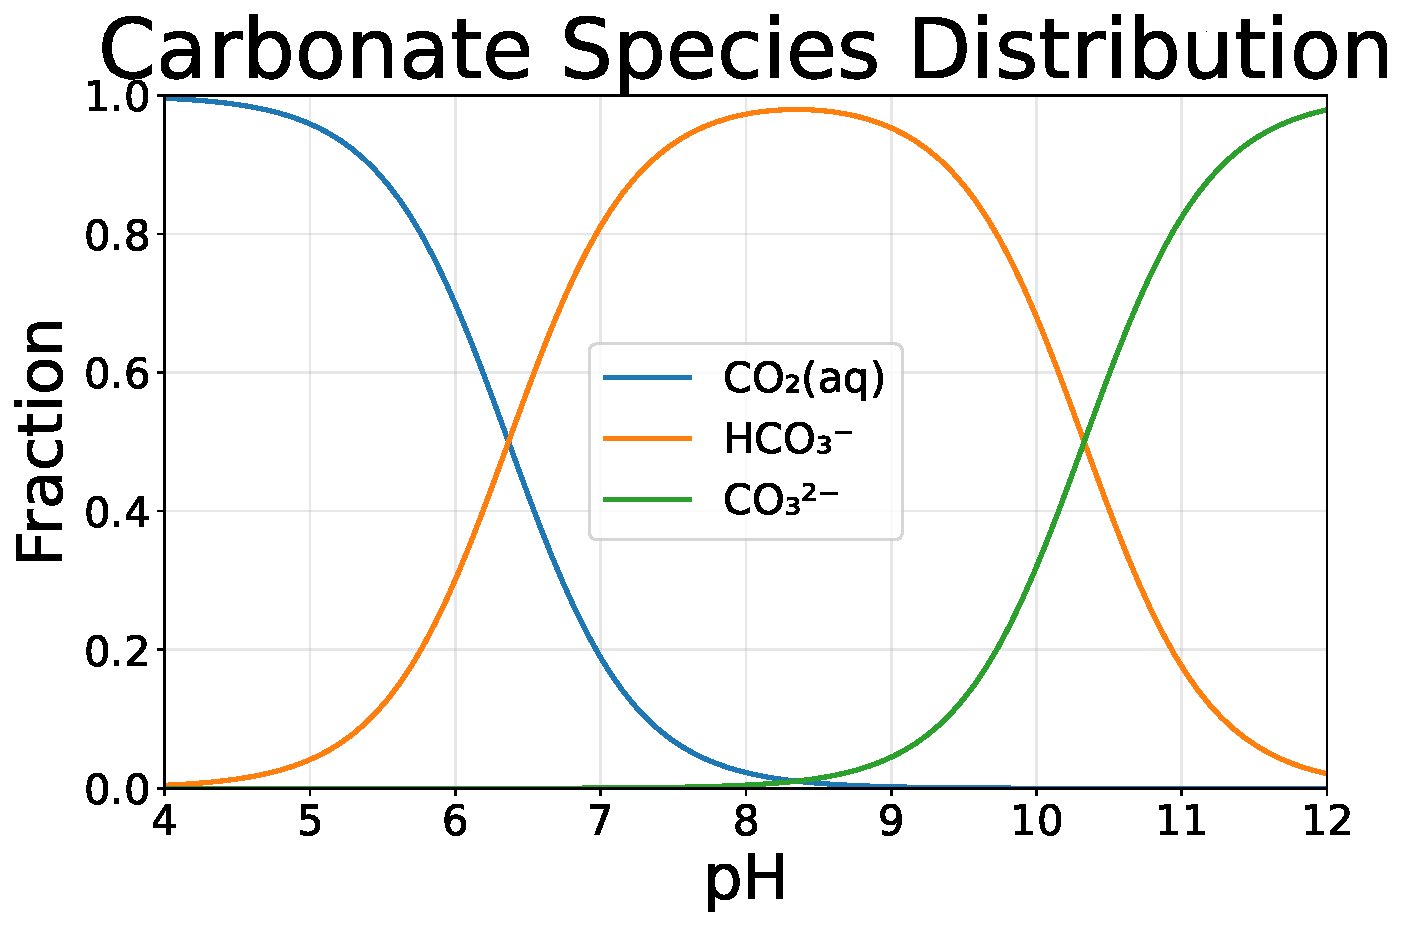
\includegraphics[scale=0.4]{/Users/fillmore/Plots/carbonate_speciation.png}
\end{figure}
\end{frame}

\begin{frame}
\begin{figure}
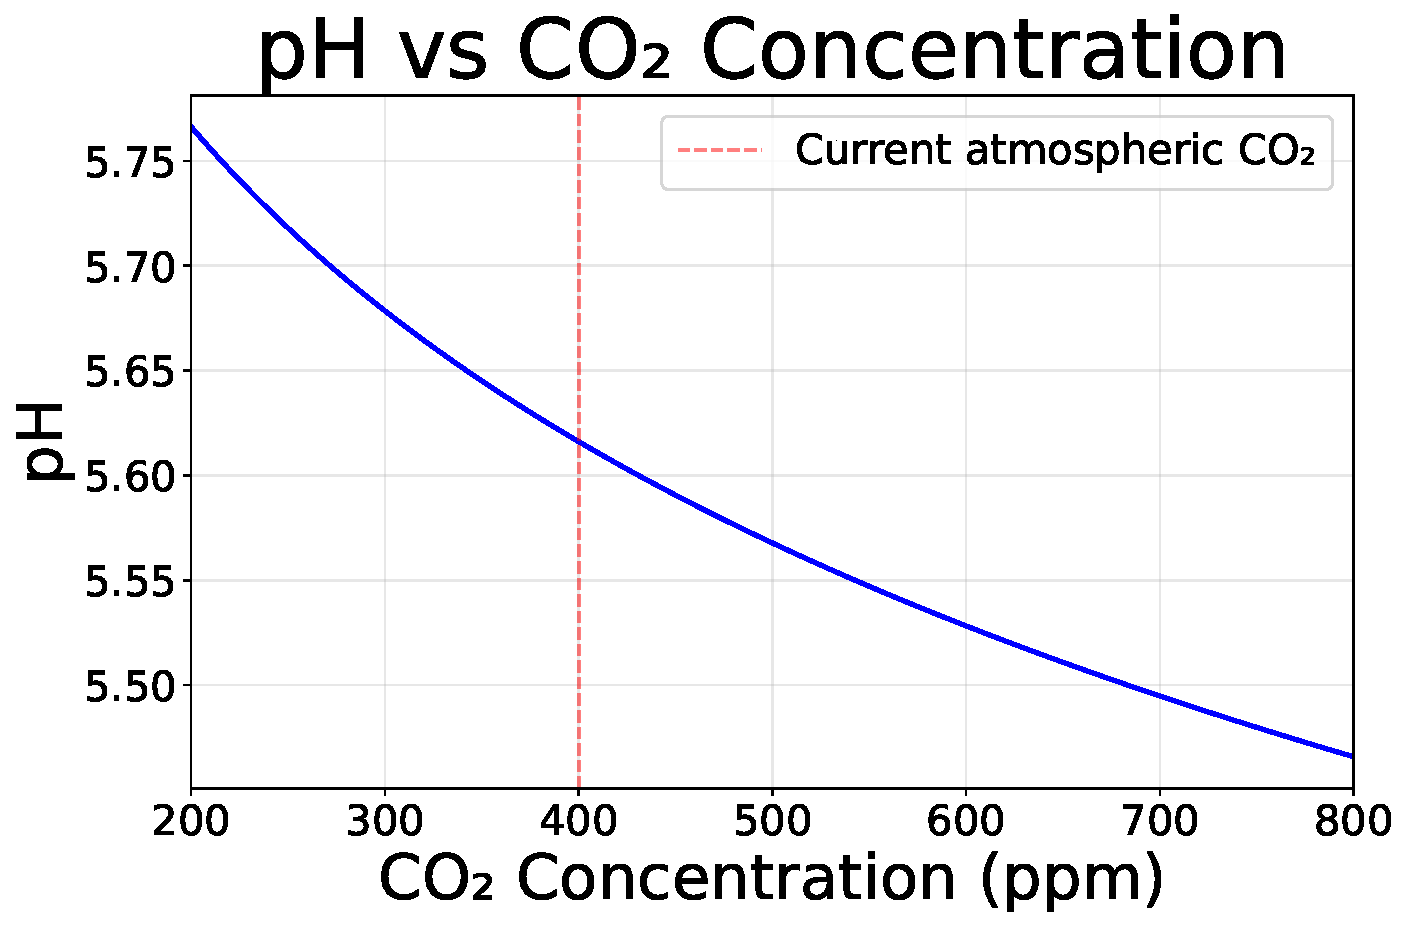
\includegraphics[scale=0.4]{/Users/fillmore/Plots/pH_vs_CO2_concentration.png}
\end{figure}
\end{frame}

\section{Differential Algebraic Equations}
\frametitle{DAE System}

\begin{frame}
\begin{block}{Variable Definitions}
\begin{align*}
x_0 &= \frac{[\ch{CO2(aq)}]}{[\ch{CO2(aq, eq)}]} \\[0.3cm]
x_1 &= \frac{[\ch{HCO3^-}]}{[\ch{HCO3^-(eq)}]} \\[0.3cm]
x_2 &= \frac{[\ch{CO3^{2-}}]}{[\ch{CO3^{2-}(eq)}]} \\[0.3cm]
y &= \frac{[\ch{H^+}]}{[\ch{H^+(eq)}]}
\end{align*}
\end{block}

\end{frame}

\begin{frame}
\vspace{-0.2in}

\begin{block}{DAE System}
\begin{align*}
\frac{dx_0}{dt} &= \frac{1}{\tau_0}[1 - x_0] \\
\frac{dx_1}{dt} &= \frac{1}{\tau_1}[x_0 - x_1 \, y(x_1, x_2)] \\
\frac{dx_2}{dt} &= \frac{1}{\tau_2}[x_1 - x_2 \, y(x_1, x_2)] \\
y(x_1, x_2) &= \frac{A}{y(x_1, x_2)} + B_1 x_1 + B_2 x_2
\end{align*}
\end{block}

\begin{block}{Analytic Solution for $x_0$}
\begin{equation*}
x_0(t) = 1 + [x_0(0) - 1]e^{-t/\tau_0}
\end{equation*}
\end{block}

\end{frame}

\begin{frame}
\begin{block}{Discretized System}
\begin{align*}
F_0 &= x_0^{n+1} - x_0^n - \frac{\Delta t}{\tau_0}[1 - x_0^{n+1}] = 0 \\[0.2cm]
F_1 &= x_1^{n+1} - x_1^n - \frac{\Delta t}{\tau_1}[x_0^{n+1} - x_1^{n+1} y^{n+1}] = 0 \\[0.2cm]
F_2 &= x_2^{n+1} - x_2^n - \frac{\Delta t}{\tau_2}[x_1^{n+1} - x_2^{n+1} y^{n+1}] = 0 \\[0.2cm]
F &= \frac{A}{y^{n+1}} + B_1 x_1^{n+1} + B_2 x_2^{n+1} - y^{n+1} = 0
\end{align*}
\end{block}

\end{frame}

\begin{frame}
\vspace{-0.15in}
\begin{block}{$\partial \mathbf{F} / \partial \mathbf{x}$}
\begin{equation*}
\frac{\partial \mathbf{F}}{\partial \mathbf{x}} = \begin{bmatrix}
1 + \frac{\Delta t}{\tau_0} & 0 & 0 \\[0.3cm]
-\frac{\Delta t}{\tau_1} & 1 + \frac{\Delta t}{\tau_1} y & 0 \\[0.3cm]
0 & -\frac{\Delta t}{\tau_2} & 1 + \frac{\Delta t}{\tau_2} y
\end{bmatrix}
\end{equation*}
\end{block}

\vspace{-0.45in}
\begin{block}{$\partial \mathbf{F} / \partial y$}
\begin{equation*}
\frac{\partial \mathbf{F}}{\partial y} = \begin{bmatrix}
0 \\[0.3cm]
\frac{\Delta t}{\tau_1} x_1 \\[0.3cm]
\frac{\Delta t}{\tau_2} x_2
\end{bmatrix}
\end{equation*}
\end{block}

\end{frame}

\begin{frame}
\vspace{-0.1in}
\begin{block}{$\partial y / \partial \mathbf{x}$}
\begin{equation*}
\frac{\partial y}{\partial \mathbf{x}} = \frac{y^2}{A + y^2} \begin{bmatrix} 0 & B_1 & B_2 \end{bmatrix}
\end{equation*}
\end{block}

\vspace{-0.3in}
\begin{block}{Total Jacobian}
\begin{equation*}
\mathbf{J} = \frac{\partial \mathbf{F}}{\partial \mathbf{x}} + \frac{\partial \mathbf{F}}{\partial y} \frac{\partial y}{\partial \mathbf{x}}
\end{equation*}
\end{block}

\end{frame}

\begin{frame}
\begin{figure}
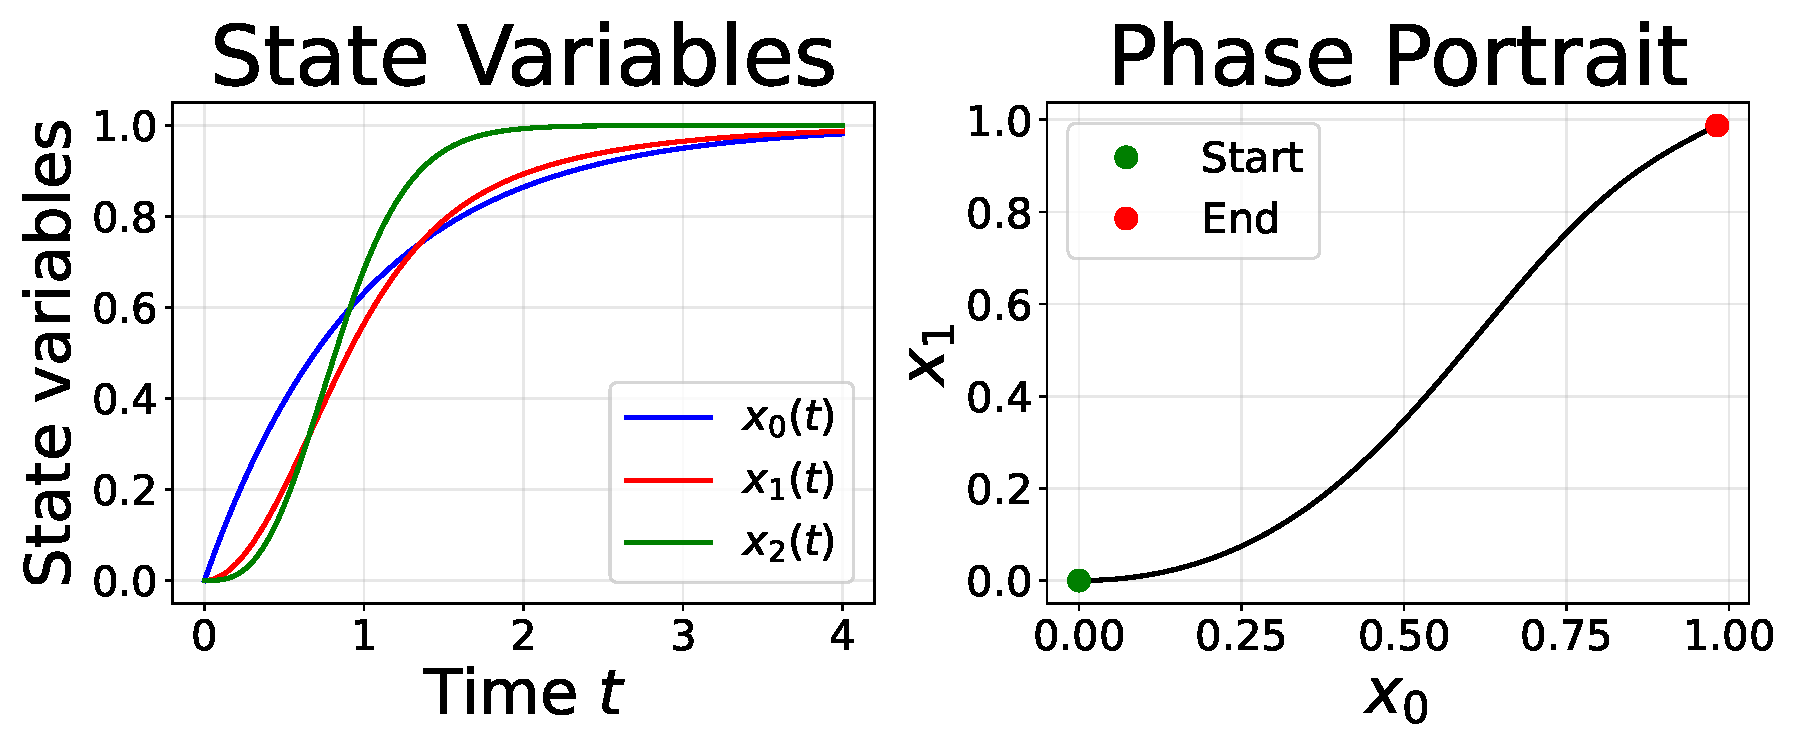
\includegraphics[scale=0.35]{/Users/fillmore/Plots/dae_system.png}
\end{figure}
\end{frame}

\end{document}
